\documentclass[11pt,oneside,letterpaper]{article}

% graphicx package, useful for including eps and pdf graphics
\usepackage{graphicx}
\DeclareGraphicsExtensions{.pdf,.png,.jpg}

% basic packages
\usepackage{color}
\usepackage{parskip}
\usepackage{float}

% text layout
\usepackage{geometry}
\geometry{textwidth=15cm} % 15.25cm for single-space, 16.25cm for double-space
\geometry{textheight=22cm} % 22cm for single-space, 22.5cm for double-space

% helps to keep figures from being orphaned on a page by themselves
\renewcommand{\topfraction}{0.85}
\renewcommand{\textfraction}{0.1}

% bold the 'Figure #' in the caption and separate it with a period
% Captions will be left justified
\usepackage[labelfont=bf,labelsep=period,font=small]{caption}

% review layout with double-spacing
%\usepackage{setspace}
%\doublespacing
%\captionsetup{labelfont=bf,labelsep=period,font=doublespacing}

% cite package, to clean up citations in the main text. Do not remove.
\usepackage{cite}
%\renewcommand\citeleft{(}
%\renewcommand\citeright{)}
%\renewcommand\citeform[1]{\textsl{#1}}

% Remove brackets from numbering in list of References
\renewcommand\refname{\large References}
\makeatletter
\renewcommand{\@biblabel}[1]{\quad#1.}
\makeatother

\usepackage{authblk}
\renewcommand\Authands{ \& }
\renewcommand\Authfont{\normalsize \bf}
\renewcommand\Affilfont{\small \normalfont}
\makeatletter
\renewcommand\AB@affilsepx{, \protect\Affilfont}
\makeatother

% notation
% \usepackage{amsmath}
% \usepackage{amssymb}

%%% TITLE %%%
\title{\vspace{1.0cm} \Large \bf
Fitness flux in SARS-CoV-2 and influenza H3N2
}

\author[1,2]{Trevor Bedford}

\affil[1]{Vaccine and Infectious Disease Division, Fred Hutchinson Cancer Center, Seattle, WA, USA}
\affil[2]{Howard Hughes Medical Institute, Seattle, WA, USA}

\date{}

\begin{document}

\maketitle

%%% ABSTRACT %%%
\begin{abstract}

TBD

\end{abstract}

\pagebreak

%%% INTRODUCTION %%%
\section*{Introduction}

TBD

%%% RESULTS %%%
\section*{Results and discussion}

% Figures
% Figure 1. Frequencies in SARS-CoV-2
% Figure 2. Fitness and mutations in SARS-CoV-2
% Figure 3. Frequencies in H3N2
% Figure 4. Fitness and mutations in H3N2
% Figure 5. Fitness variance vs fitness flux in SARS-CoV-2
% Figure 6. Fitness variance vs fitness flux in H3N2
% Figure 7. Pango tree (panel A) and Pango branch distributions (panel B)
% Figure 8. Scatterplot correlations between mutations and fitness
% Supp Figure Y. Scatterplot correlation of EvEscape and fitness

Description of MLR model and cumulative fitness flux.
Rate of evolution of SARS-CoV-2 in terms of fitness flux and in terms of S1 mutations.
Rate of evolution of H3N2 in terms of fitness flux and in terms of S1 mutations.

%%% sarscov2_clades_frequencies %%%
\begin{figure}[h]
	\centering
	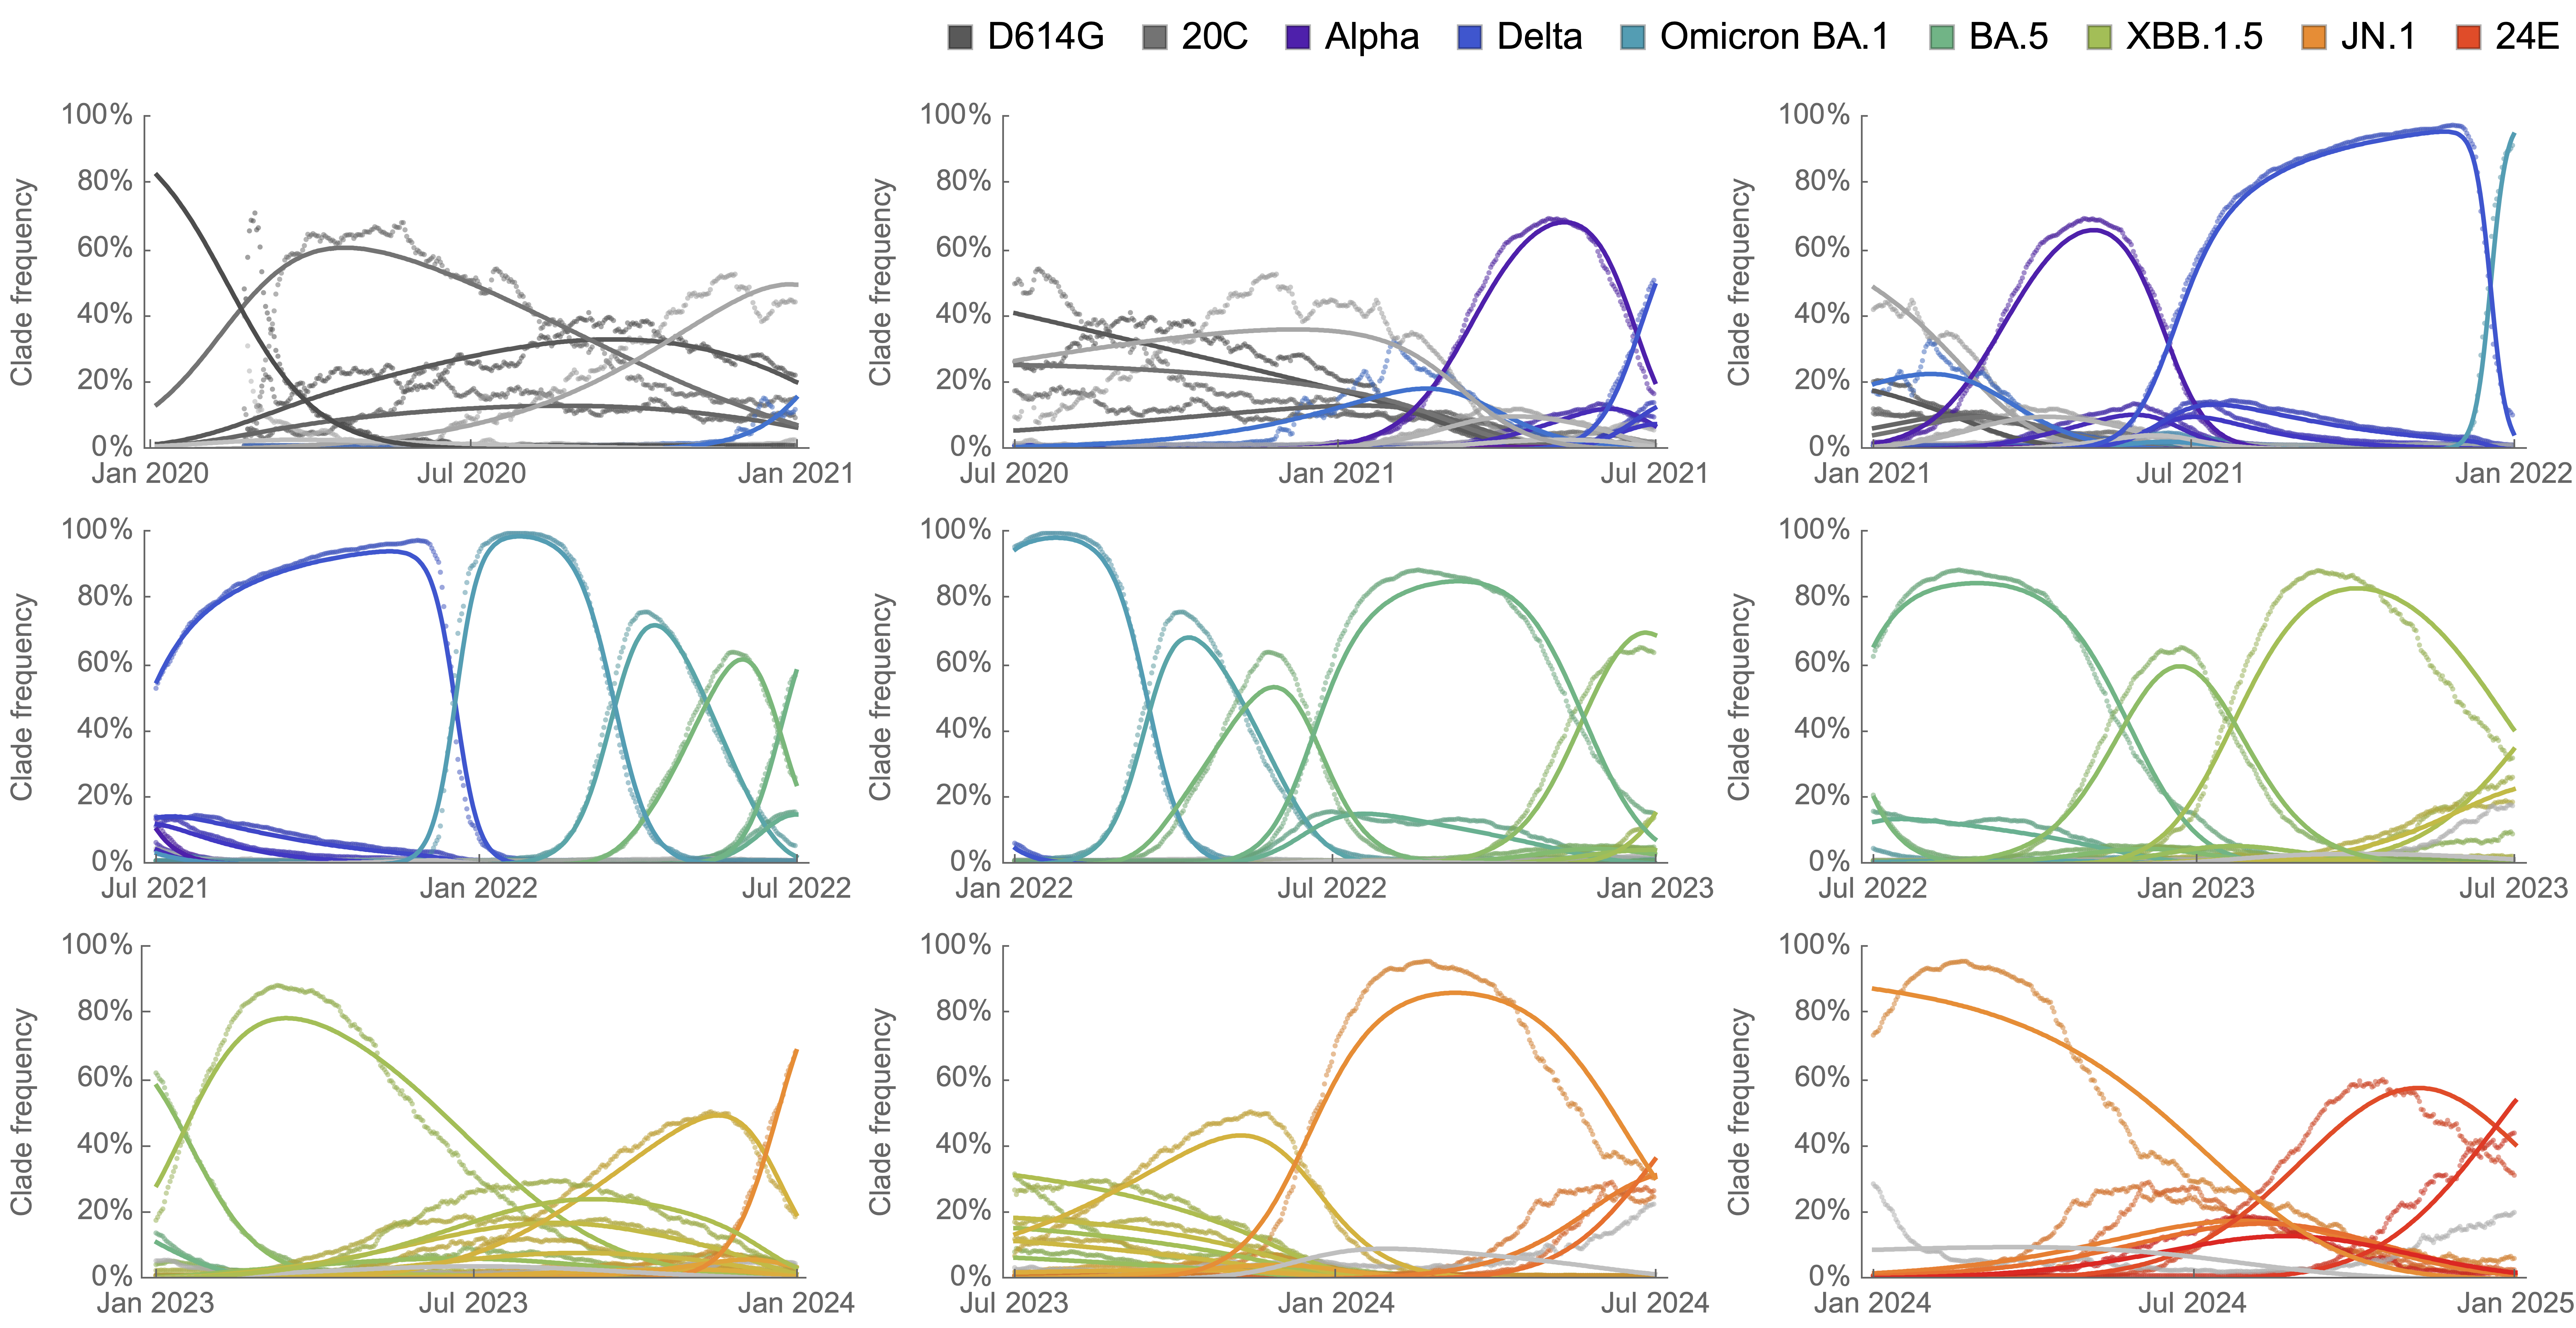
\includegraphics[width=1.0\textwidth]{figures/sarscov2_clades_frequencies}
	\caption{\textbf{Relative frequencies of SARS-CoV-2 clades through time.}
  Points represent empirical frequencies of SARS-CoV-2 Nextstrain clades, while solid lines represent modeled frequencies from Multinomial Logistic Regression (MLR).
	All data is taken from the USA.
  The MLR analysis assumes that the fitness of each clade is constant through time.
	}
	\label{sarscov2_clades_frequencies}
\end{figure}

%%% sarscov2_clades_fitnesses_mutations %%%
\begin{figure}[h]
	\centering
	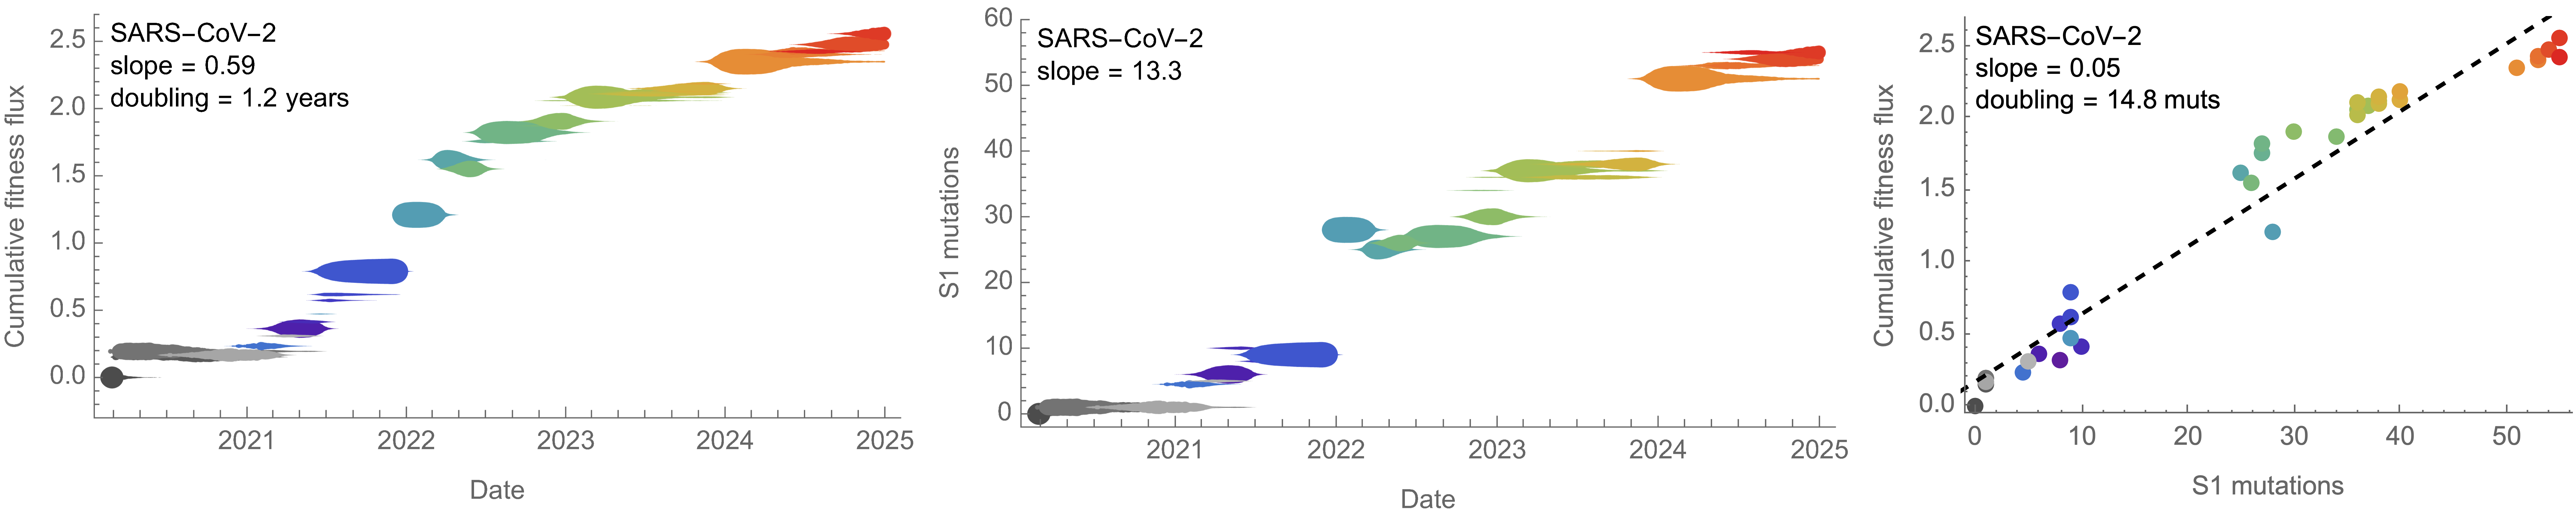
\includegraphics[width=1.0\textwidth]{figures/sarscov2_clades_fitnesses_mutations}
	\caption{\textbf{Cumulative SARS-CoV-2 fitness flux and spike S1 mutations.}
  (A) Empirical frequencies of SARS-CoV-2 Nextstrain clades are represented by vertical thickness and placement on the y-axis represents cumulative fitness flux estimated from Multinomial Logistic Regression (MLR).
  (B) As before, empirical frequencies of SARS-CoV-2 clades are represented by vertical thickness, though placement on the y-axis represents cumulative median spike S1 mutations in viruses belonging to each clade.
  (C) Cumulative spike S1 mutations plotted against cumulative fitness flux across SARS-CoV-2 clades.
	All data is taken from the USA.
  The MLR analysis assumes that the fitness of each clade is constant through time.
	}
	\label{sarscov2_clades_fitnesses_mutations}
\end{figure}

%%% h3n2_clades_frequencies %%%
\begin{figure}[h]
	\centering
	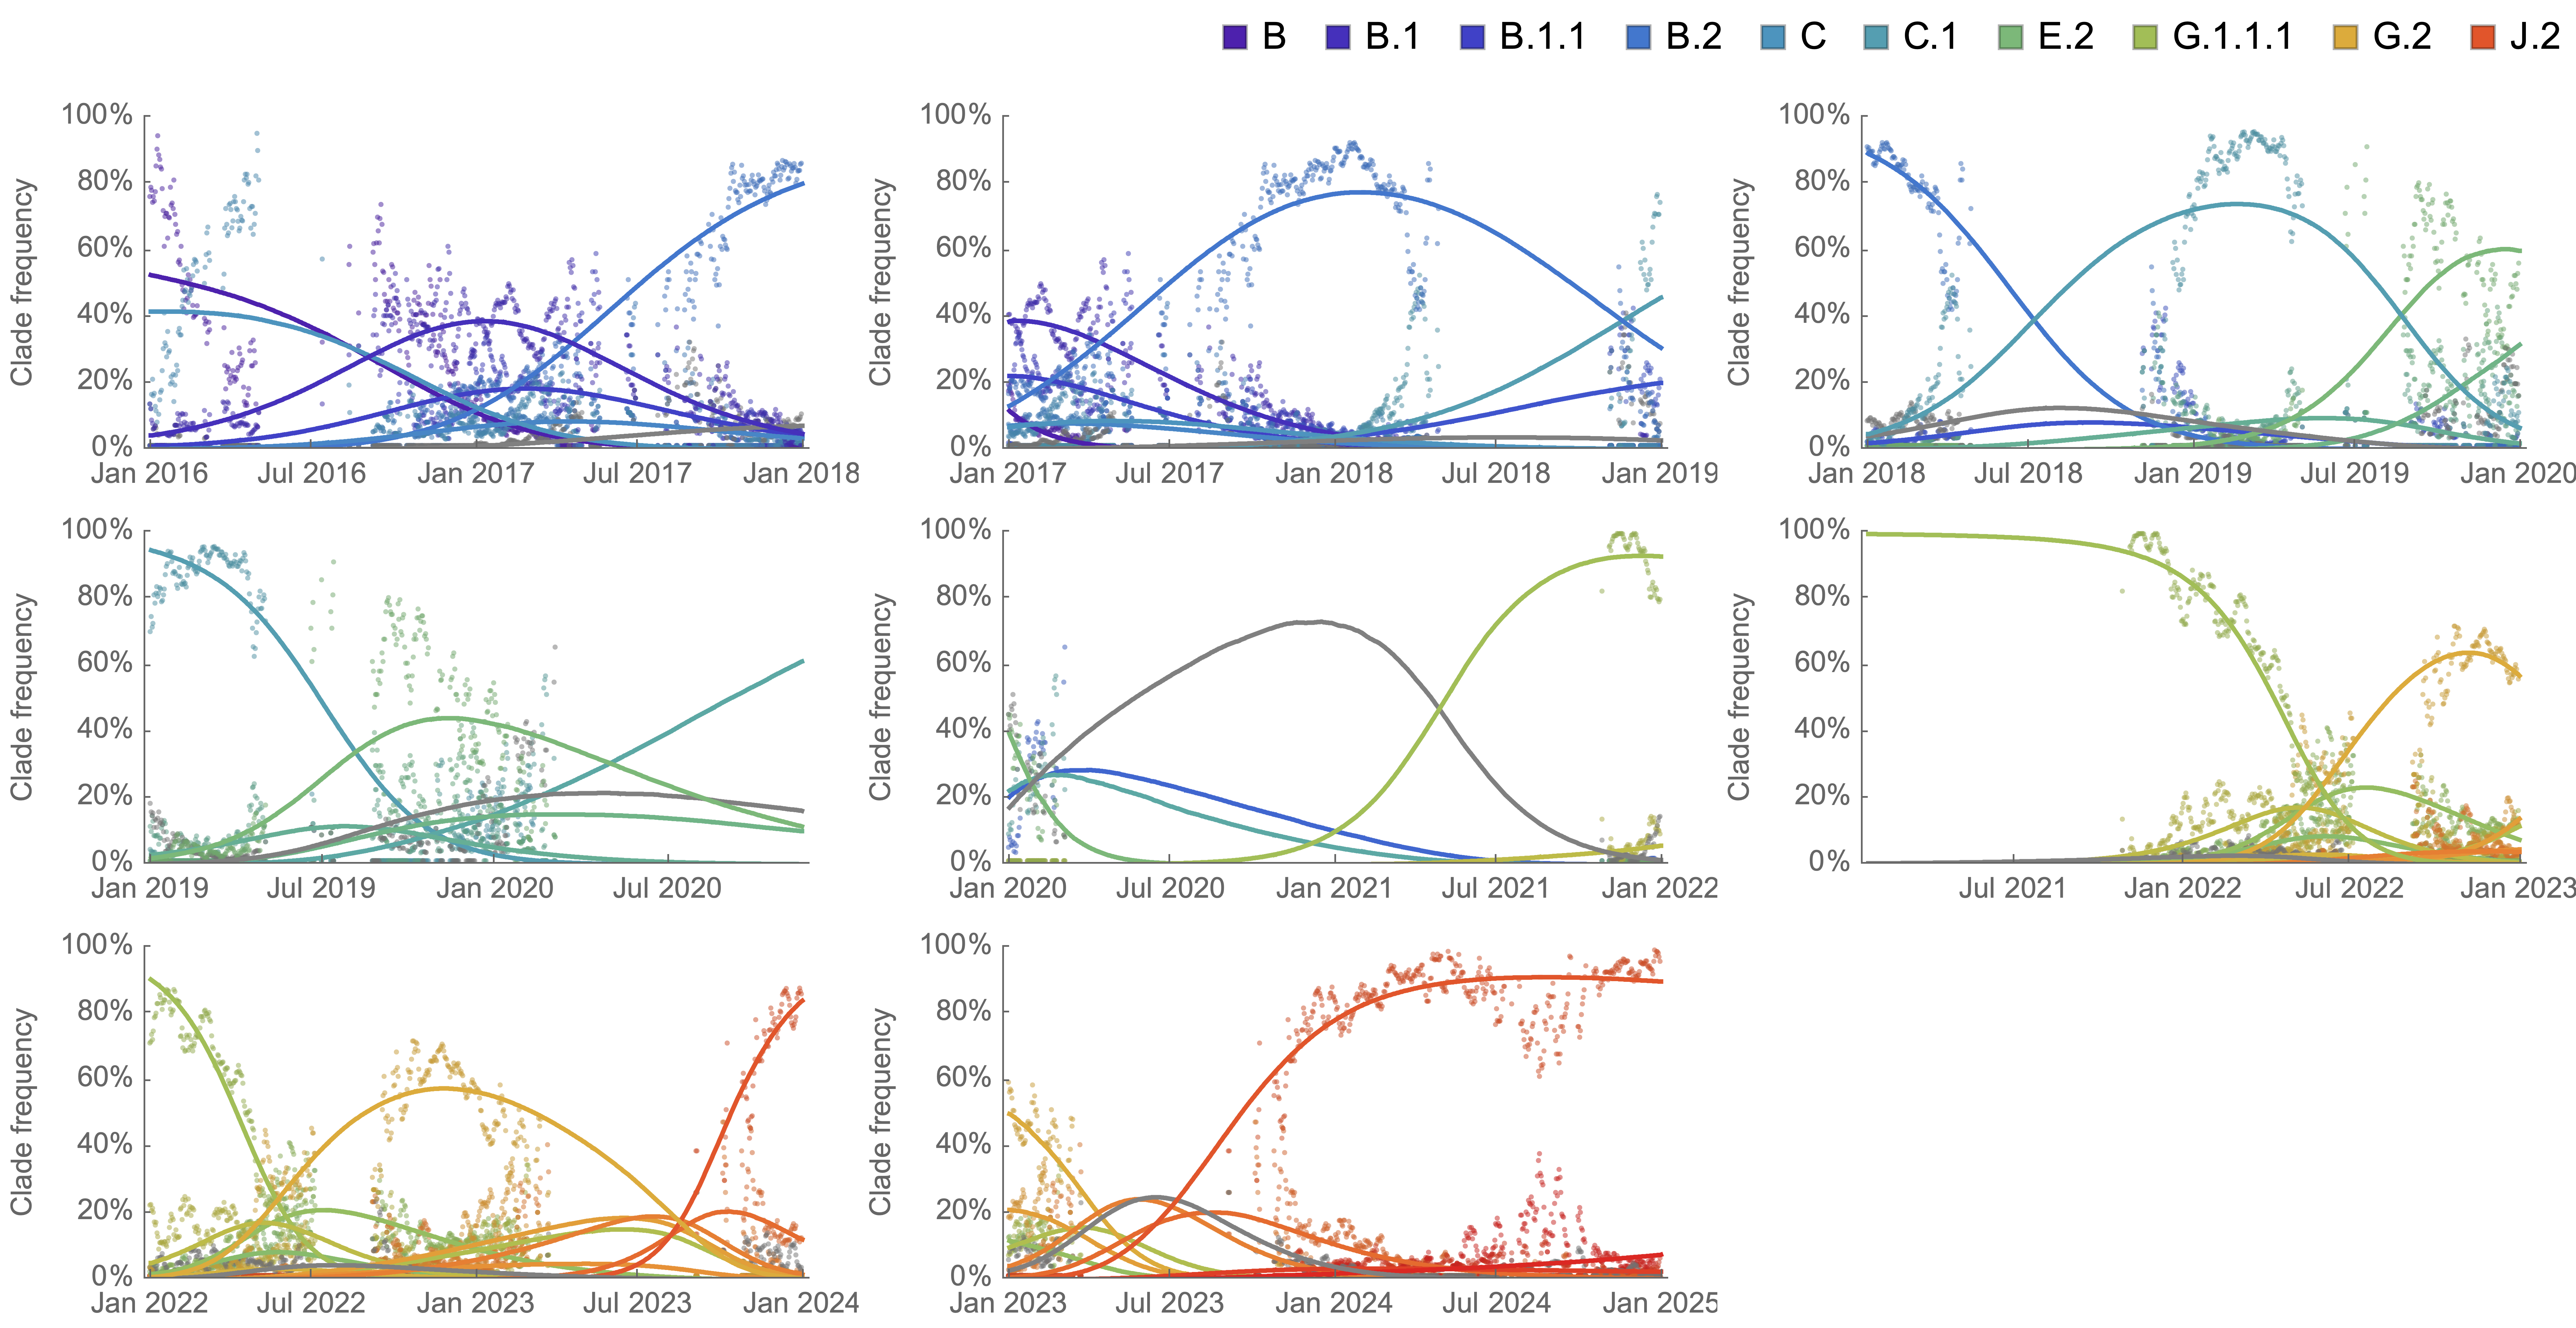
\includegraphics[width=1.0\textwidth]{figures/h3n2_clades_frequencies}
	\caption{\textbf{Relative frequencies of H3N2 clades through time.}
  Points represent empirical frequencies of H3N2 Nextstrain clades, while solid lines represent modeled frequencies from Multinomial Logistic Regression (MLR).
	All data is taken from the USA.
  The MLR analysis assumes that the fitness of each clade is constant through time.
	}
	\label{h3n2_clades_frequencies}
\end{figure}

%%% h3n2_clades_fitnesses_mutations %%%
\begin{figure}[h]
	\centering
	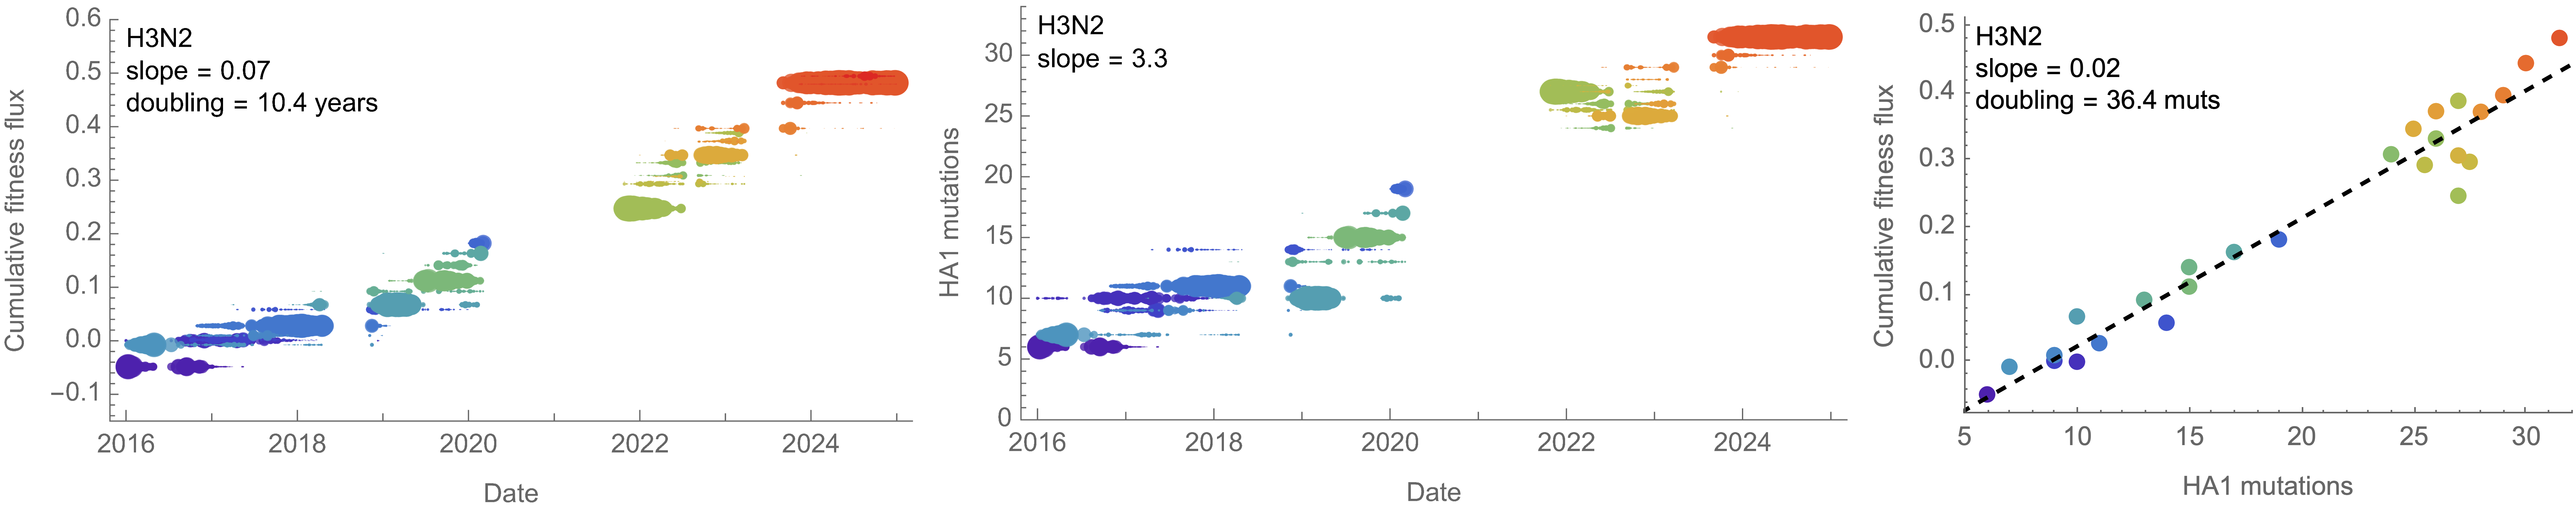
\includegraphics[width=1.0\textwidth]{figures/h3n2_clades_fitnesses_mutations}
	\caption{\textbf{Cumulative H3N2 fitness flux and spike S1 mutations.}
  (A) Empirical frequencies of H3N2 Nextstrain clades are represented by vertical thickness and placement on the y-axis represents cumulative fitness flux estimated from Multinomial Logistic Regression (MLR).
  (B) As before, empirical frequencies of H3N2 clades are represented by vertical thickness, though placement on the y-axis represents cumulative median spike S1 mutations in viruses belonging to each clade.
  (C) Cumulative spike S1 mutations plotted against cumulative fitness flux across H3N2 clades.
	All data is taken from the USA.
  The MLR analysis assumes that the fitness of each clade is constant through time.
	}
	\label{h3n2_clades_fitnesses_mutations}
\end{figure}

Fisher's fundemental theorem and the expected relationship of fitness variance and fitness flux.
Empirical investigation of this relationship in SARS-CoV-2 and H3N2.

%%% sarscov2_clades_fitness_variance_vs_flux %%%
\begin{figure}[h]
	\centering
	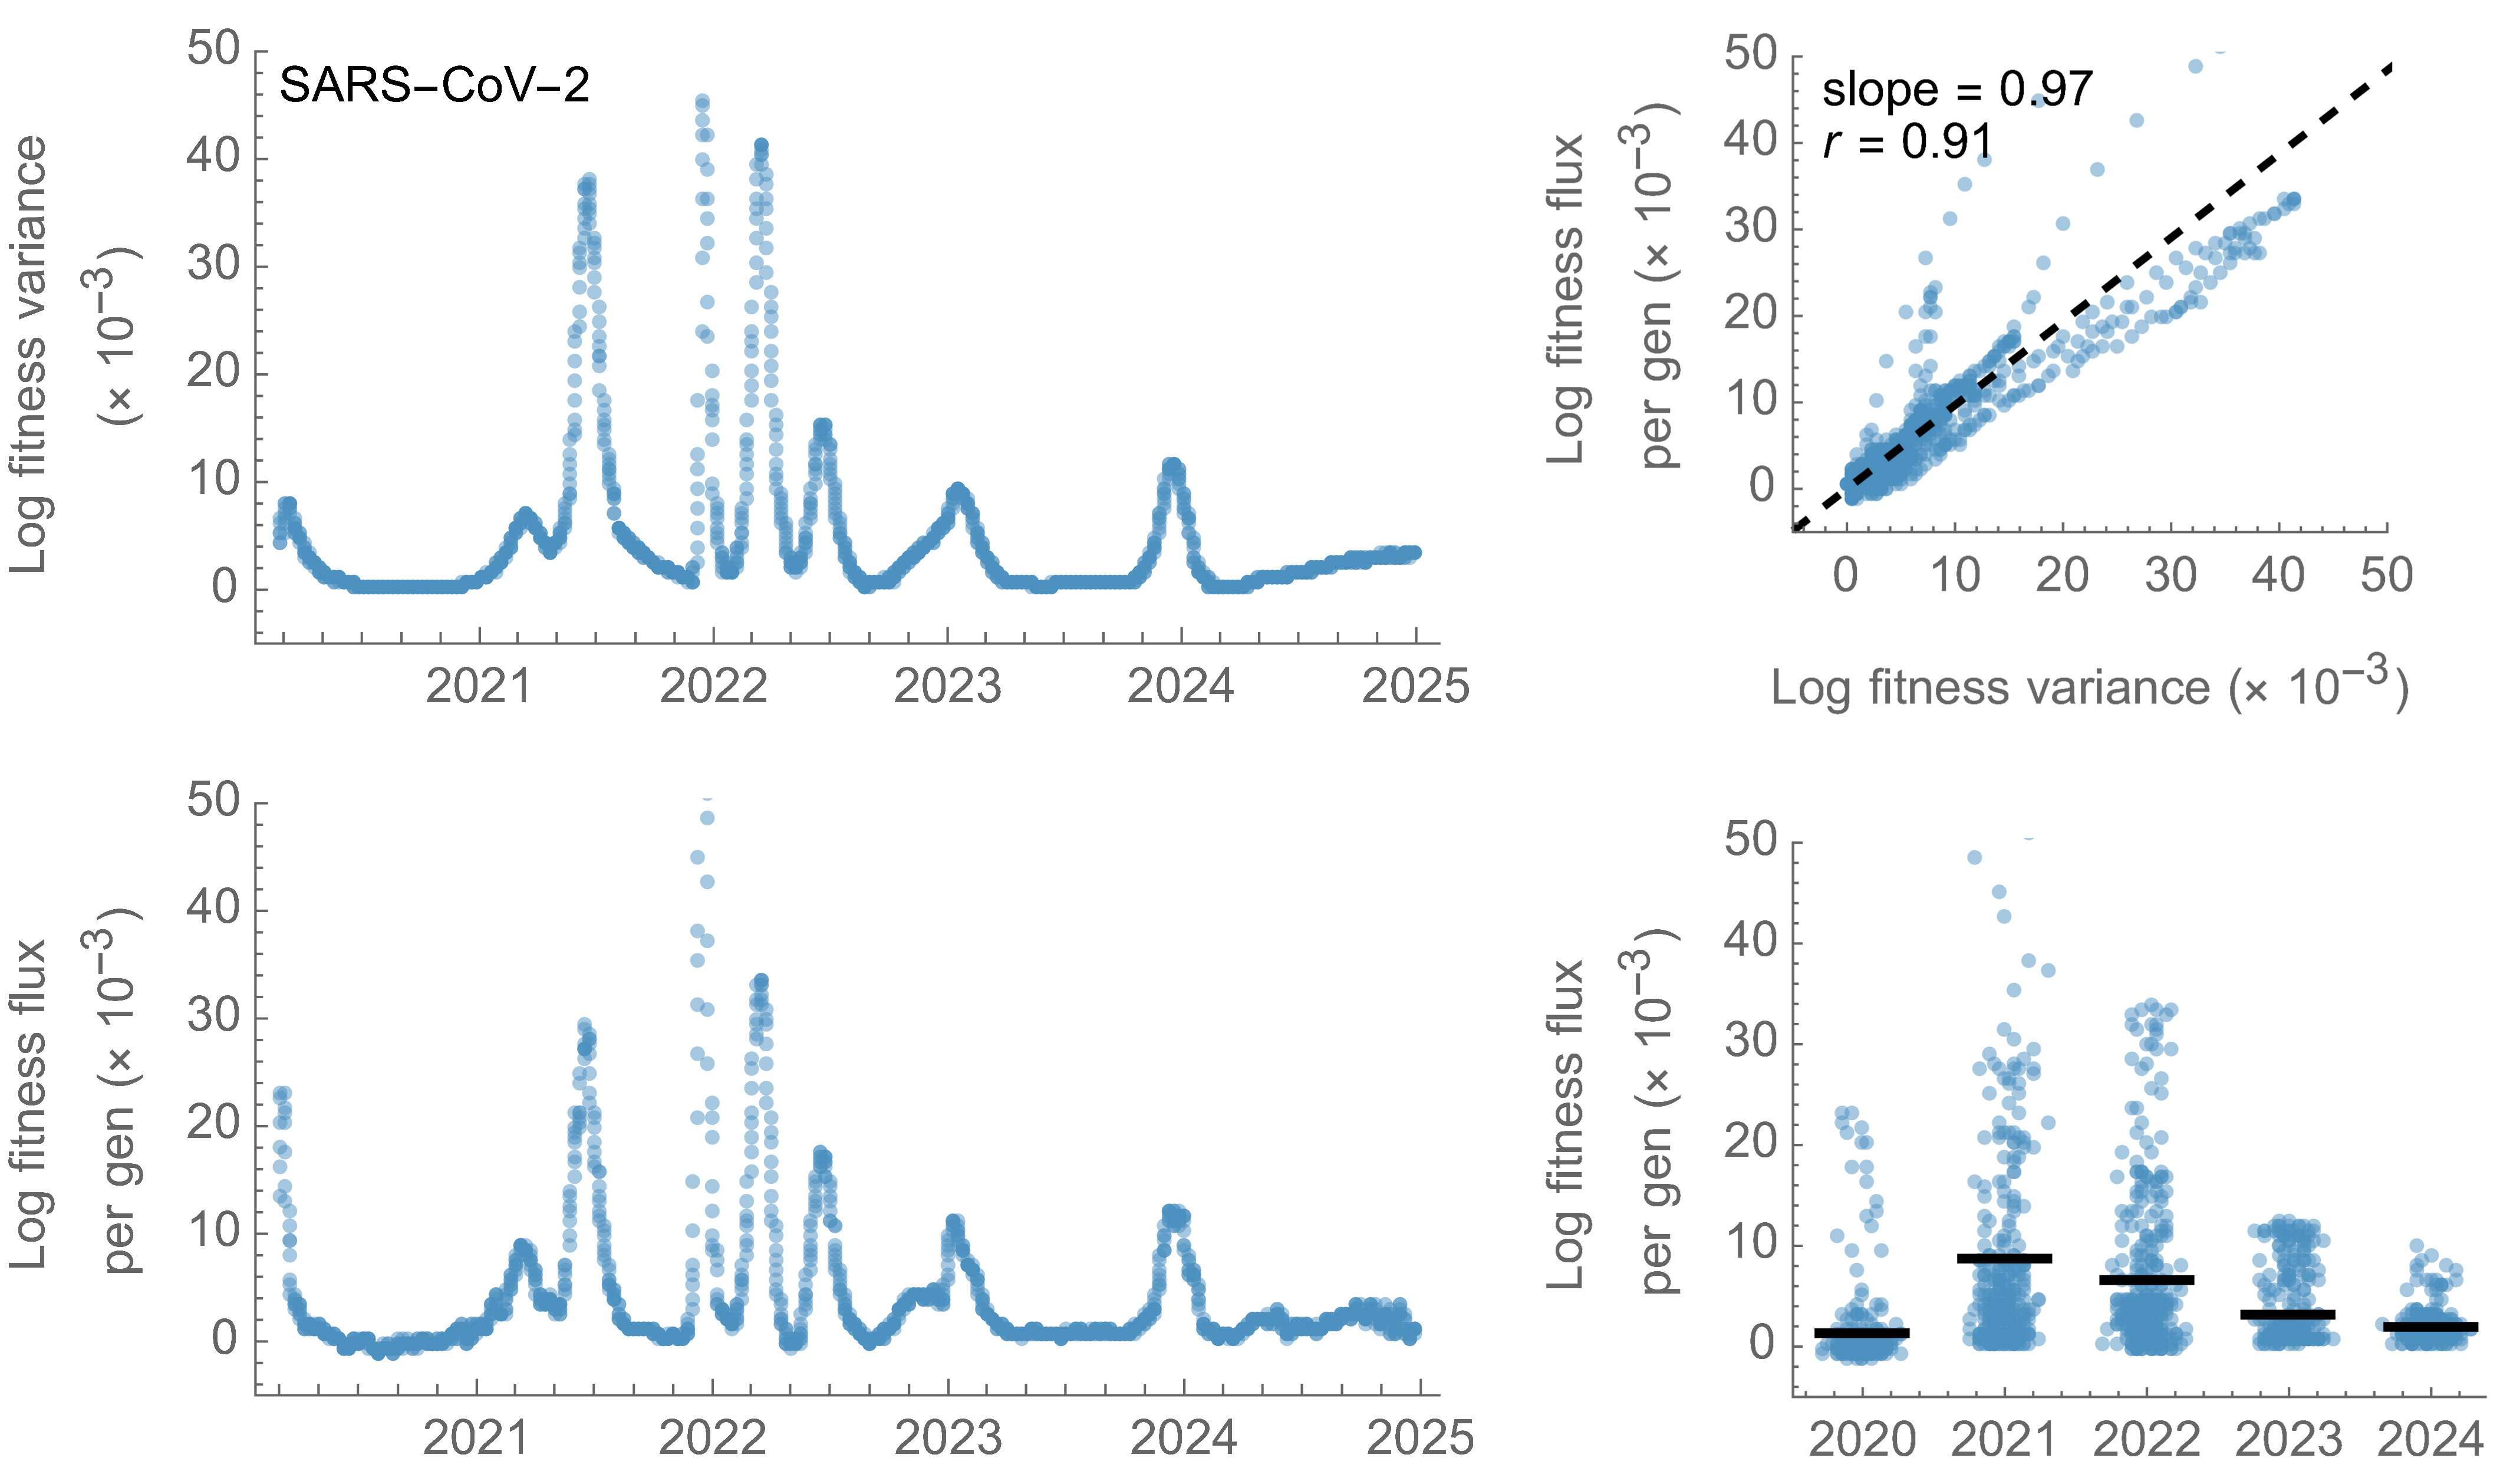
\includegraphics[width=1.0\textwidth]{figures/sarscov2_clades_fitness_variance_vs_flux}
	\caption{\textbf{Fitness variance and fitness flux in SARS-CoV-2.}
  Log fitness variance is comparabled to log fitness flux, where each dot represents a daily timepoint.
	}
	\label{sarscov2_clades_fitness_variance_vs_flux}
\end{figure}

%%% h3n2_clades_fitness_variance_vs_flux %%%
\begin{figure}[h]
	\centering
	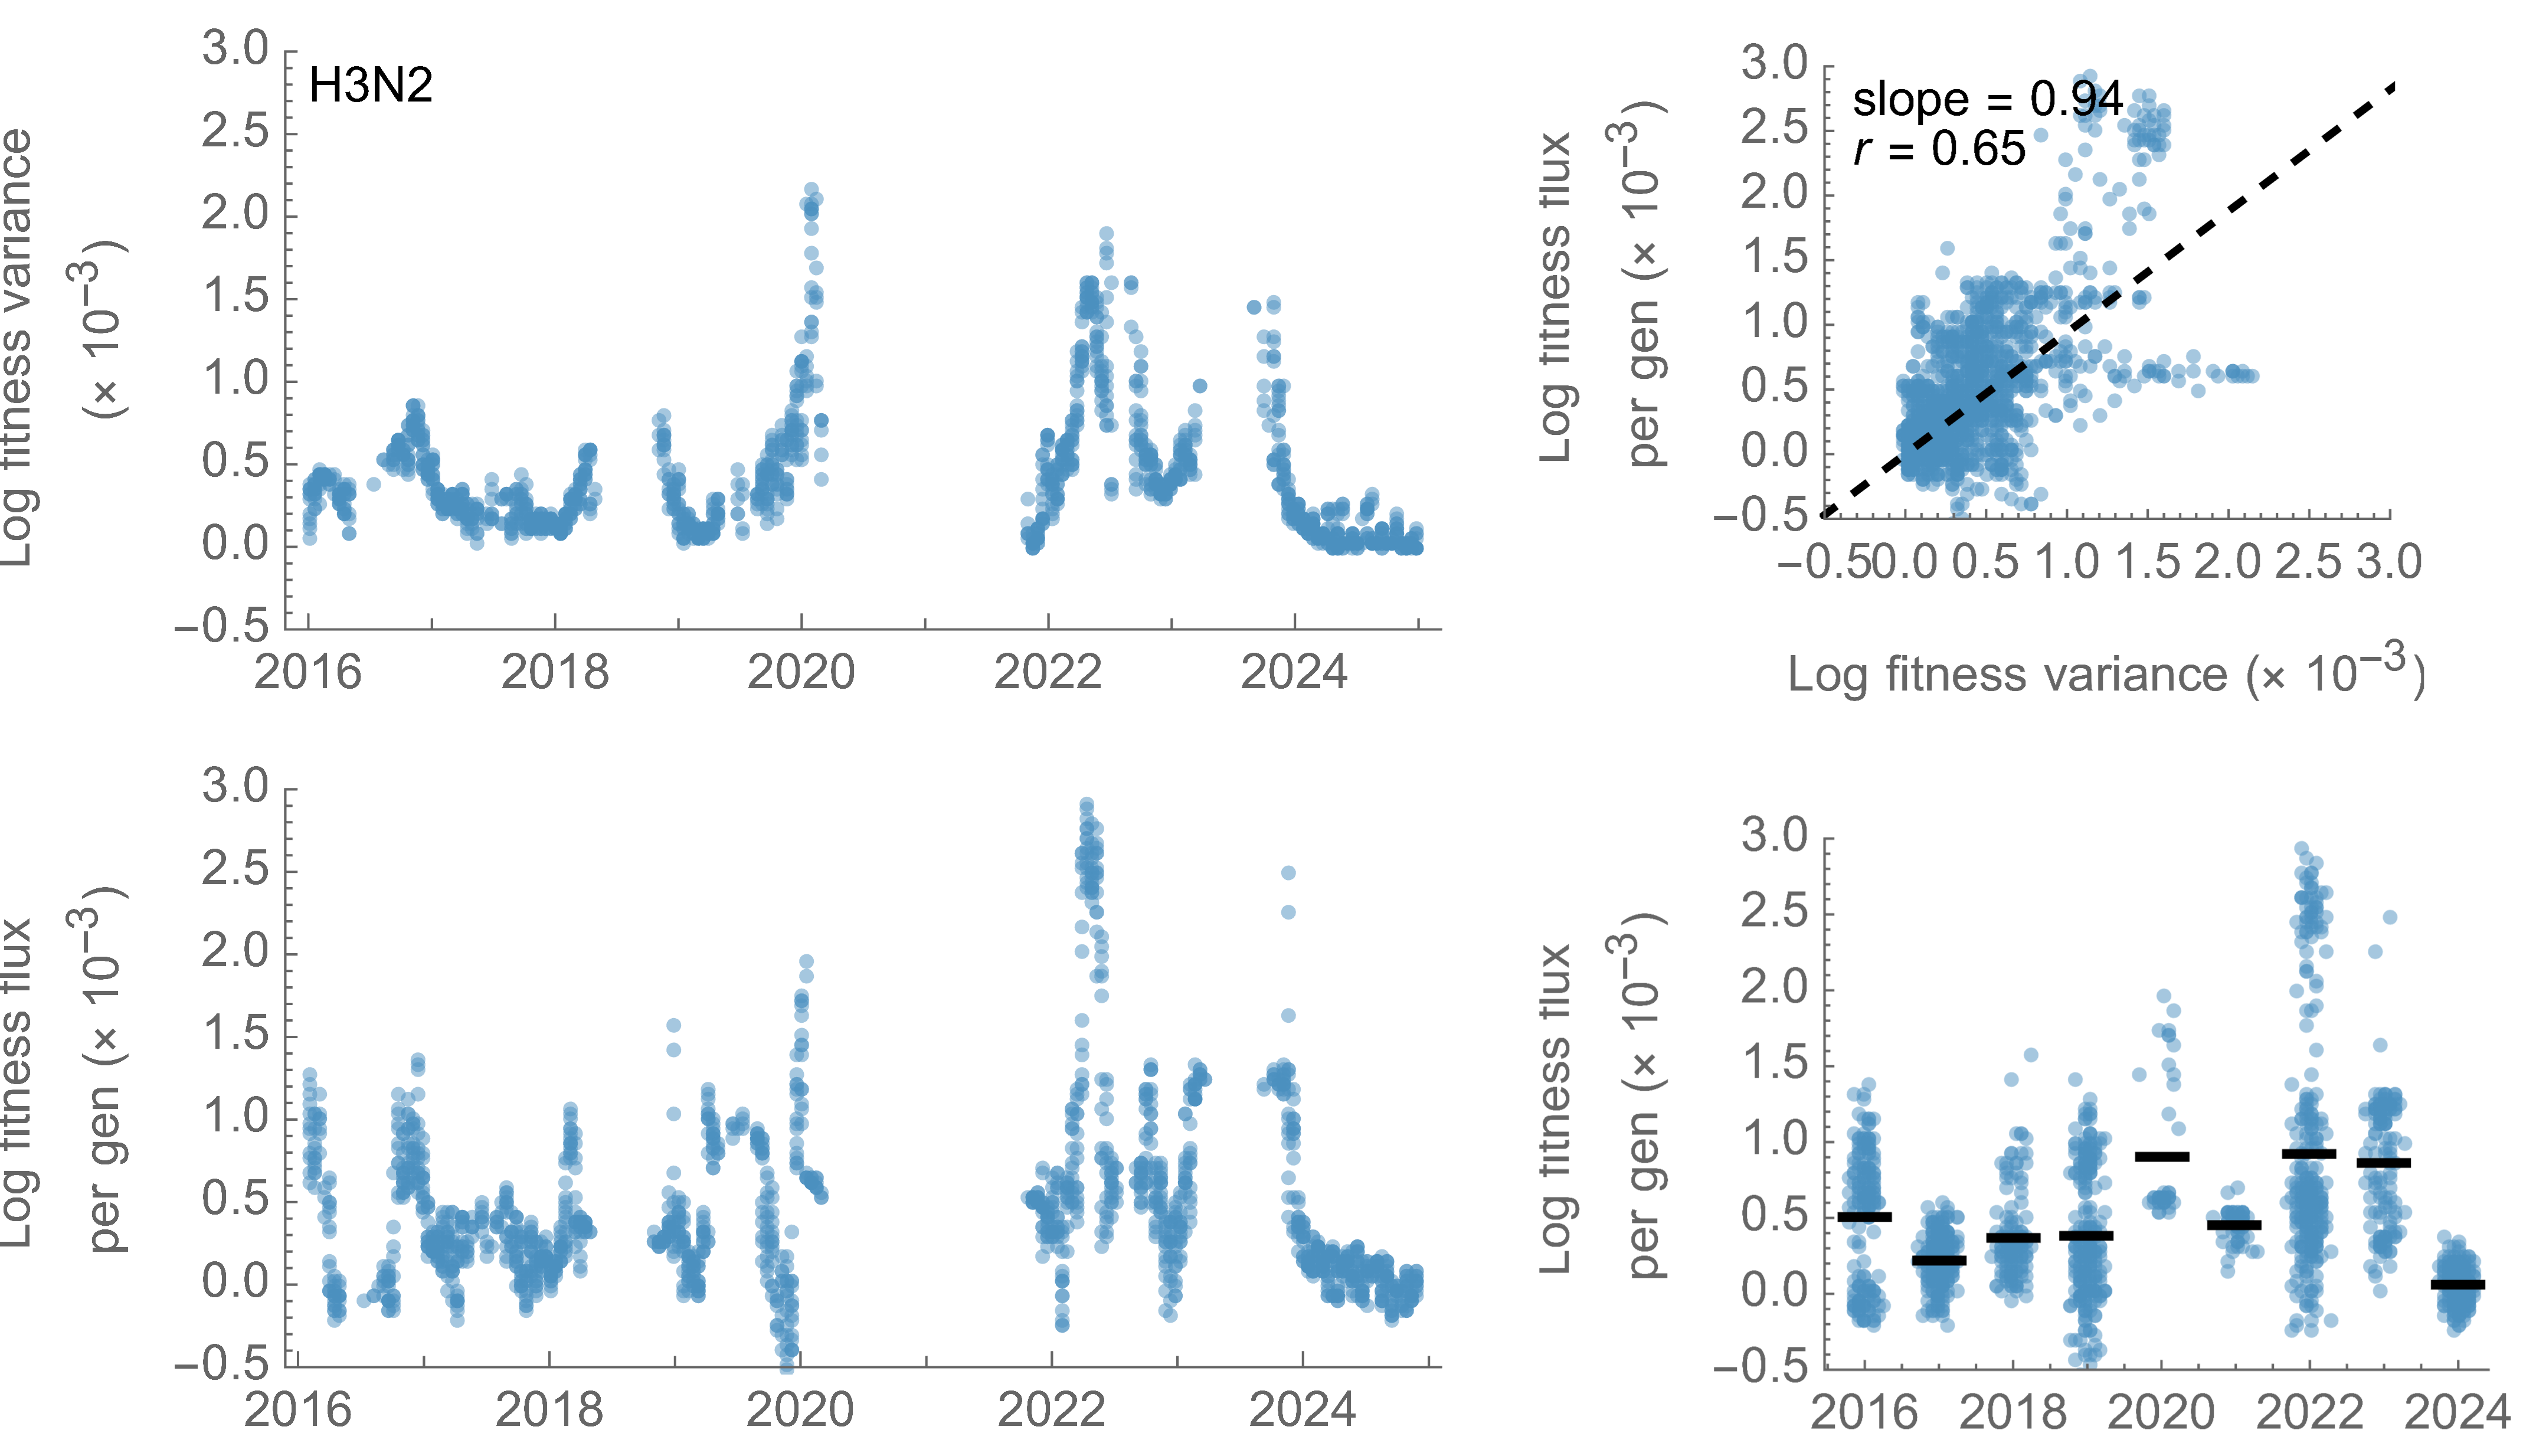
\includegraphics[width=1.0\textwidth]{figures/h3n2_clades_fitness_variance_vs_flux}
	\caption{\textbf{Fitness variance and fitness flux in H3N2.}
  Log fitness variance is comparabled to log fitness flux, where each dot represents a daily timepoint.
	}
	\label{h3n2_clades_fitness_variance_vs_flux}
\end{figure}

We shouldn't do a simple correlation of mutations against cumulative fitness flux due to phylogenetic non-independence.
Instead can rely on phylogenetic contrasts of parent and daughter lineages.
Pango lineages provide a convenient granular and hierarchical nomenclature well suited to this.

%%% sarscov2_lineage_delta_fitness_across_genome %%%
\begin{figure}[h]
	\centering
	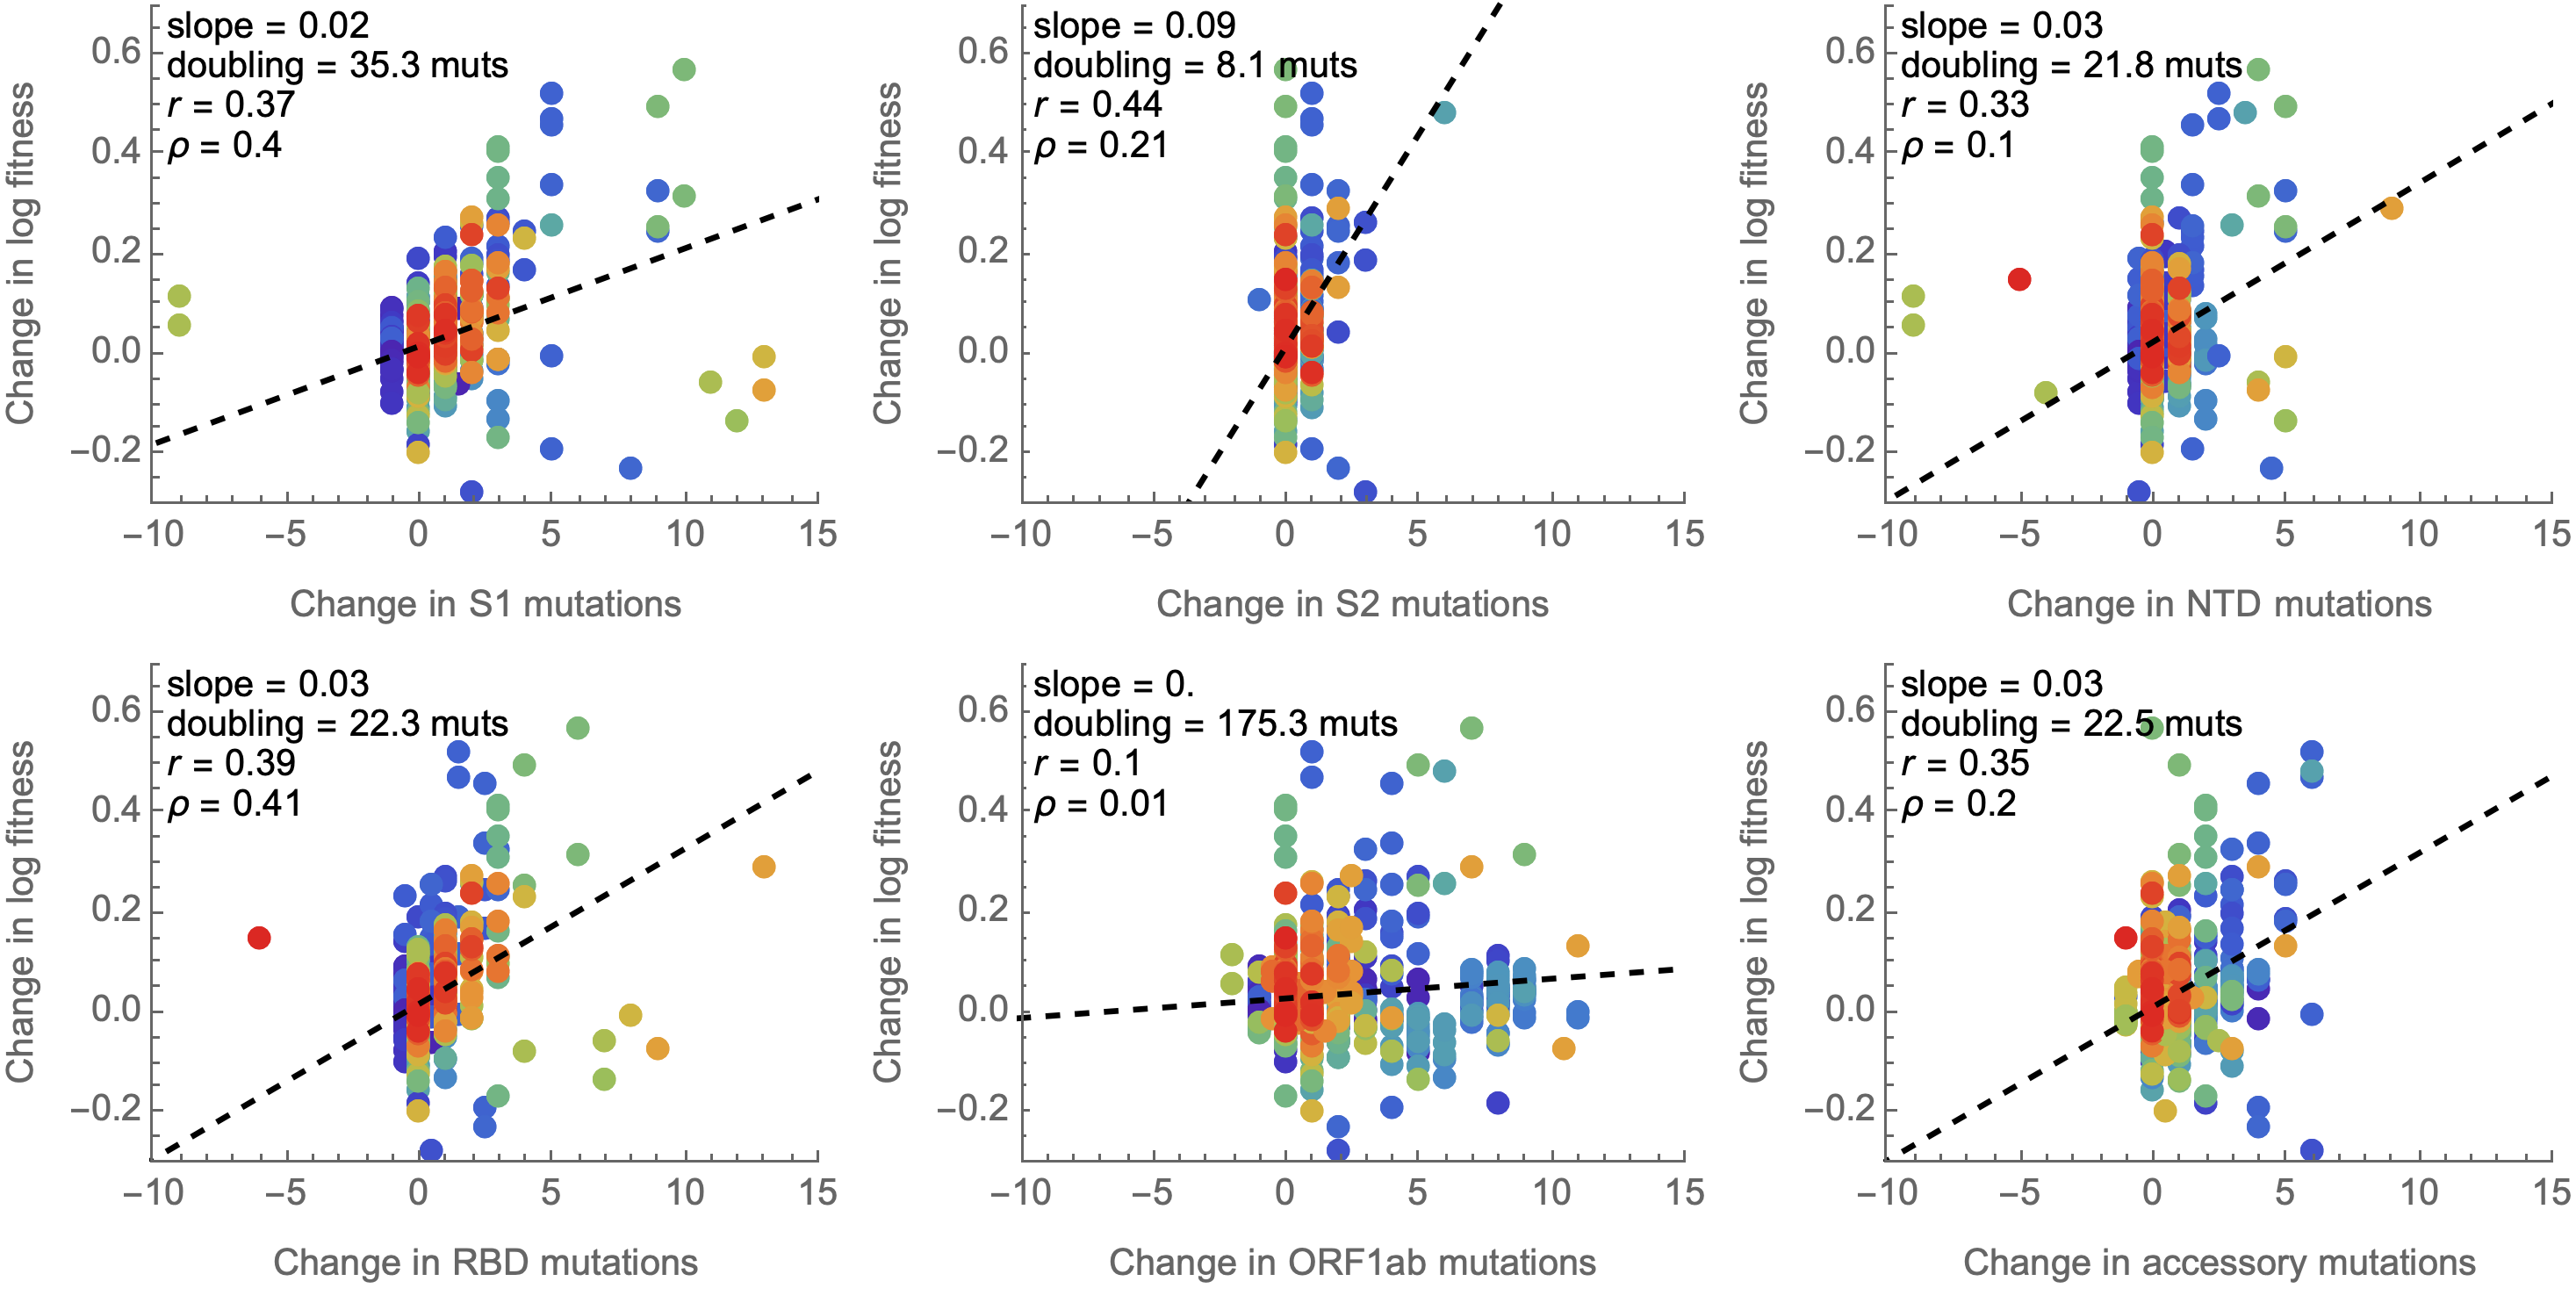
\includegraphics[width=1.0\textwidth]{figures/sarscov2_lineage_delta_fitness_across_genome}
	\caption{\textbf{Correlation of lineage-specific amino acid change to lineage-specific fitness change across regions of the SARS-CoV-2 genome.}
	}
	\label{sarscov2_lineage_delta_fitness_across_genome}
\end{figure}

%%% sarscov2_lineage_delta_fitness_across_time %%%
\begin{figure}[h]
	\centering
	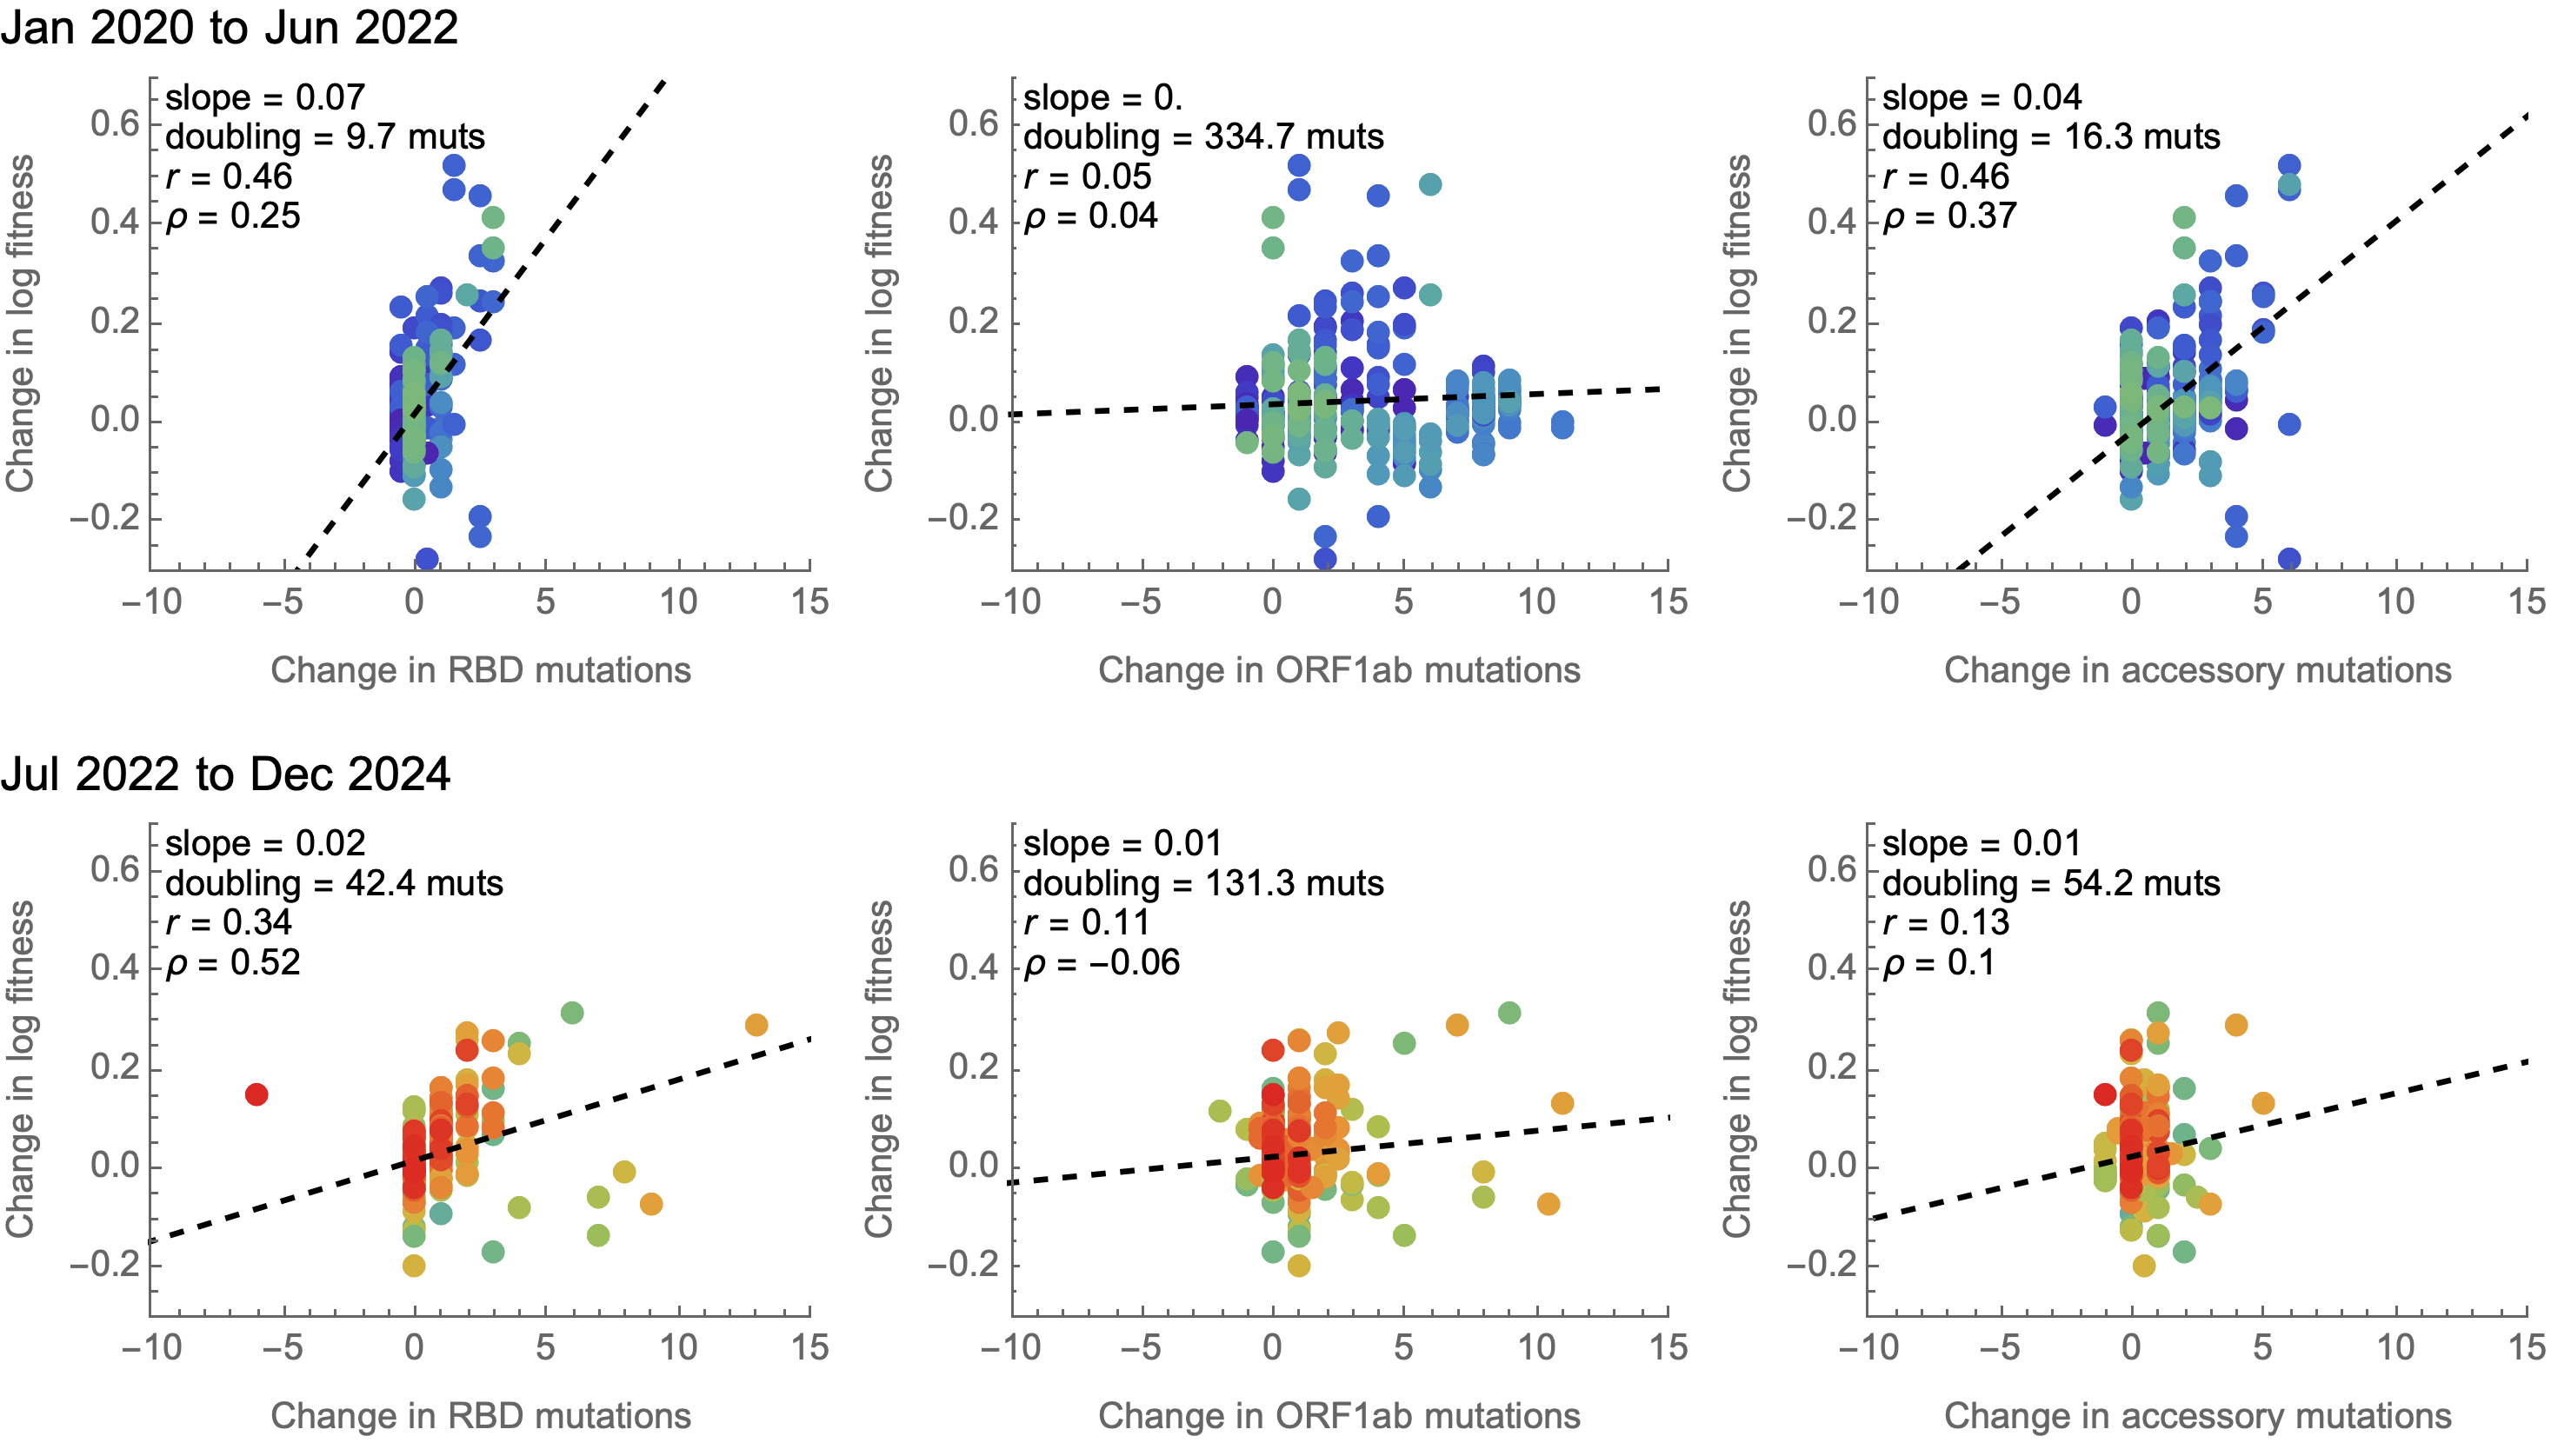
\includegraphics[width=1.0\textwidth]{figures/sarscov2_lineage_delta_fitness_across_time}
	\caption{\textbf{Correlation of lineage-specific amino acid change to lineage-specific fitness change over time.}
	}
	\label{sarscov2_lineage_delta_fitness_across_time}
\end{figure}

%%% sarscov2_lineage_delta_fitness_vs_evescape %%%
\begin{figure}[h]
	\centering
	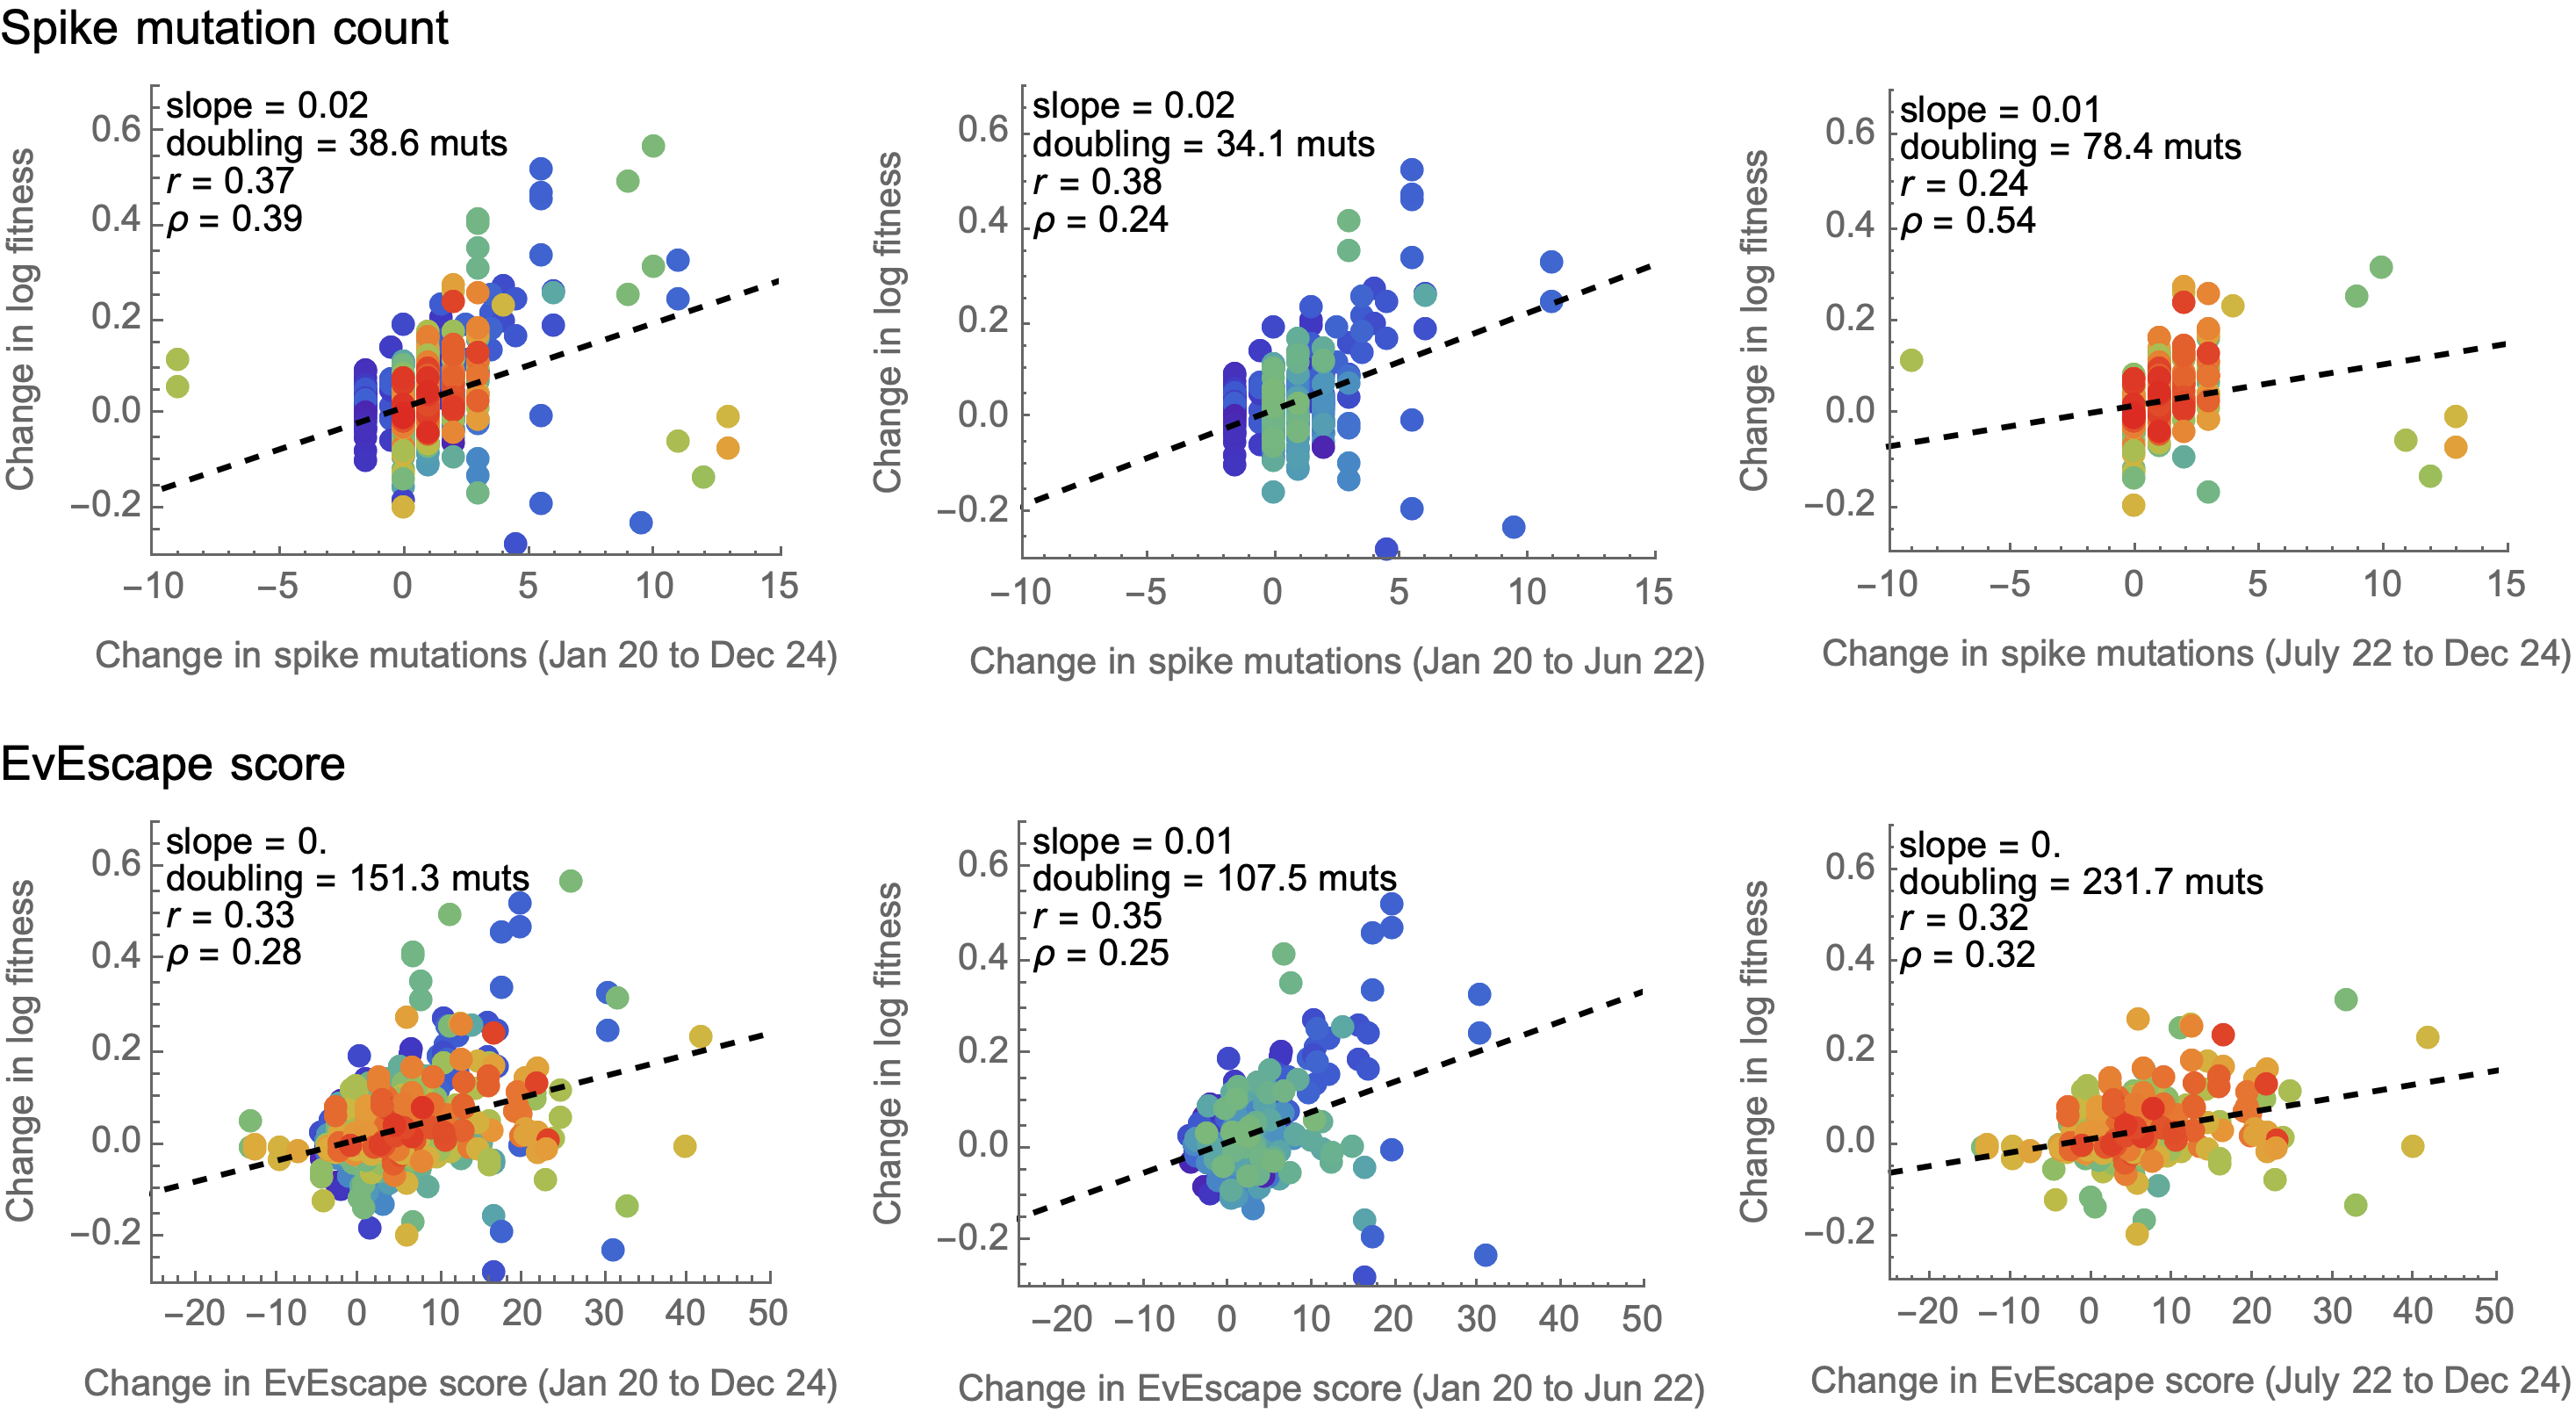
\includegraphics[width=1.0\textwidth]{figures/sarscov2_lineage_delta_fitness_vs_evescape}
	\caption{\textbf{Correlation of lineage-specific change in EvEscape score to lineage-specific fitness change.}
	}
	\label{sarscov2_lineage_delta_fitness_vs_evescape}
\end{figure}

%%% CONCLUSIONS %%%
\section*{Conclusions}

TBD

%%% METHODS %%%
\section*{Materials and methods}

TBD

%%% ACKNOWLEDGMENTS %%%
\subsection*{Acknowledgments}

TBD

%%% REFERENCES %%%
\bibliographystyle{plos}
\bibliography{fitness_flux}

\end{document}
